\documentclass[10pt,a4paper]{article}
\usepackage[margin=1.8cm]{geometry}
\usepackage[T1]{fontenc}
\usepackage{lmodern,microtype,amsmath,booktabs,multirow,graphicx,xcolor,caption,enumitem}
\usepackage[colorlinks=true,linkcolor=blue!50!black,urlcolor=blue!50!black,citecolor=blue!50!black]{hyperref}
\captionsetup{font=small,labelfont=bf}
\setlist{nosep,leftmargin=1.2em}
\setlength{\parskip}{3pt}
\setlength{\emergencystretch}{2em}
\graphicspath{{../results/figures/}}

\title{\vspace{-1.2cm}Homework 1: Image Enhancement\\[2pt]\large Computer Vision -- Fall 2026}
\author{Kazi Hasnayeen Emad}
\date{}

\begin{document}
\maketitle
\vspace{-1.0cm}

\noindent\textbf{Repository:} \url{https://github.com/YOUR-USERNAME/hw1-image-enhancement}
\hfill (code, images, results, \texttt{metrics.csv}, README)

\section{Objective and data}
The goal is to build and compare a small classical (no deep learning) pipeline that enhances colour images
affected by low contrast, non-uniform illumination and noise, and to analyse the trade-offs between
visibility of details, noise and natural appearance.

\textbf{Images.} We use five of the author's own smartphone photographs of outdoor scenes (no synthetic images).
\textbf{Source and licence:} own photographs, taken by the author and redistributed by the author in the
repository (\texttt{data/raw/}). For speed, each 1932$\times$2576 photo is downsampled to 720$\times$960 px with
area interpolation (\texttt{src/prepare\_data.py}); these PNGs are the originals.

\begin{center}\footnotesize
\begin{tabular}{@{}ll@{}}
\toprule
Image & Condition exhibited\\\midrule
\texttt{forest} & dark, back-lit forest canopy; sun in frame with lens flare; shadowed trunks\\
\texttt{waterfall\_haze} & haze and back-light; dark vegetation behind the falls; sun rays\\
\texttt{river\_boat} & atmospheric haze, low contrast on the distant hillside\\
\texttt{waterfall\_canyon} & harsh sunlight with deep shadows in the gorge (non-uniform illumination)\\
\texttt{hut} & large bright sky vs.\ darker hillside and ground; haze\\
\bottomrule
\end{tabular}
\end{center}

\textbf{Synthetic degradation.} For reproducible evaluation each original $I$ is degraded as
\[
I_d=\operatorname{clip}_{[0,255]}\!\big(\operatorname{round}(\mu + c\,(I-\mu) + n)\big),\qquad c=0.5,\quad n\sim\mathcal N(0,6^2),
\]
where $\mu$ is the global mean of $I$ (brightness is preserved, the dynamic range is halved) and $n$ is i.i.d.\ per
pixel and channel, generated with \texttt{numpy.random.default\_rng(42+k)} for the $k$-th image. Both versions are
saved. \emph{The original images serve only as references for evaluating these synthetic degradations; in
real-world scenarios a clean reference is generally not available.} Because the contraction is applied in RGB
around a grey level, it also reduces colour saturation (e.g.\ mean Lab chroma of \texttt{hut}: 25.0\,$\rightarrow$\,14.9,
OpenCV 8-bit units), which matters in the discussion.

\section{Methods and parameters}
All methods take the degraded 8-bit image and use OpenCV \cite{opencv} and NumPy (\texttt{src/enhance.py});
background in \cite{gw}. Data, degradations and evaluation settings are identical for every method.
\begin{enumerate}
\item \textbf{Baseline}: the degraded image, unprocessed.
\item \textbf{Linear contrast stretching}: the $[p_1,p_{99}]$ percentile range is mapped linearly to $[0,255]$
(1\% saturated at each end, robust to noise outliers). Main variant: on \textbf{luminance} $L^*$ of CIE-Lab with
$a^*,b^*$ unchanged, so hue is preserved and no colour cast is introduced. For comparison we also stretch
\textbf{per channel} (B, G, R independently): each channel gets its own gain/offset, which acts like an automatic
white balance and can shift colours.
\item \textbf{Histogram equalisation}: global \texttt{cv2.equalizeHist} on $L^*$, chroma unchanged. Equalising
$L^*$ instead of R, G, B avoids hue shifts, but since $a^*,b^*$ stay fixed while $L^*$ changes strongly, perceived
saturation changes (darkened areas look more saturated, brightened ones paler).
\item \textbf{Fourth method -- NLM denoising + luminance stretch} (motivated combination). Stretching multiplies the
noise by the same gain as the signal (about $1/c=2\times$ here), so we denoise \emph{before} amplifying, with
non-local means \cite{buades2005}, \texttt{cv2.fastNlMeansDenoisingColored} ($h=h_\text{color}=4$, template 7,
search 21), then apply method 2 on $L^*$. Noise reduction necessarily also smooths fine texture.
\end{enumerate}

\textbf{Metrics} (\texttt{src/metrics.py}), on the degraded set against the original: \textbf{PSNR} (own
implementation, peak 255, all pixels and channels), \textbf{SSIM} \cite{wang2004} (scikit-image \cite{skimage},
Gaussian window $\sigma=1.5$, mean over channels) and \textbf{MAE} in grey levels.

\section{Results}
Figure~\ref{fig:grid} shows the side-by-side comparison for every image and method, all on the same fixed
$[0,255]$ display scale; Fig.~\ref{fig:crops} shows 1:1 crops where noise and fine detail are visible;
Table~\ref{tab:m} reports the metrics (also in \texttt{results/metrics.csv}).

\begin{figure}[!ht]
\centering
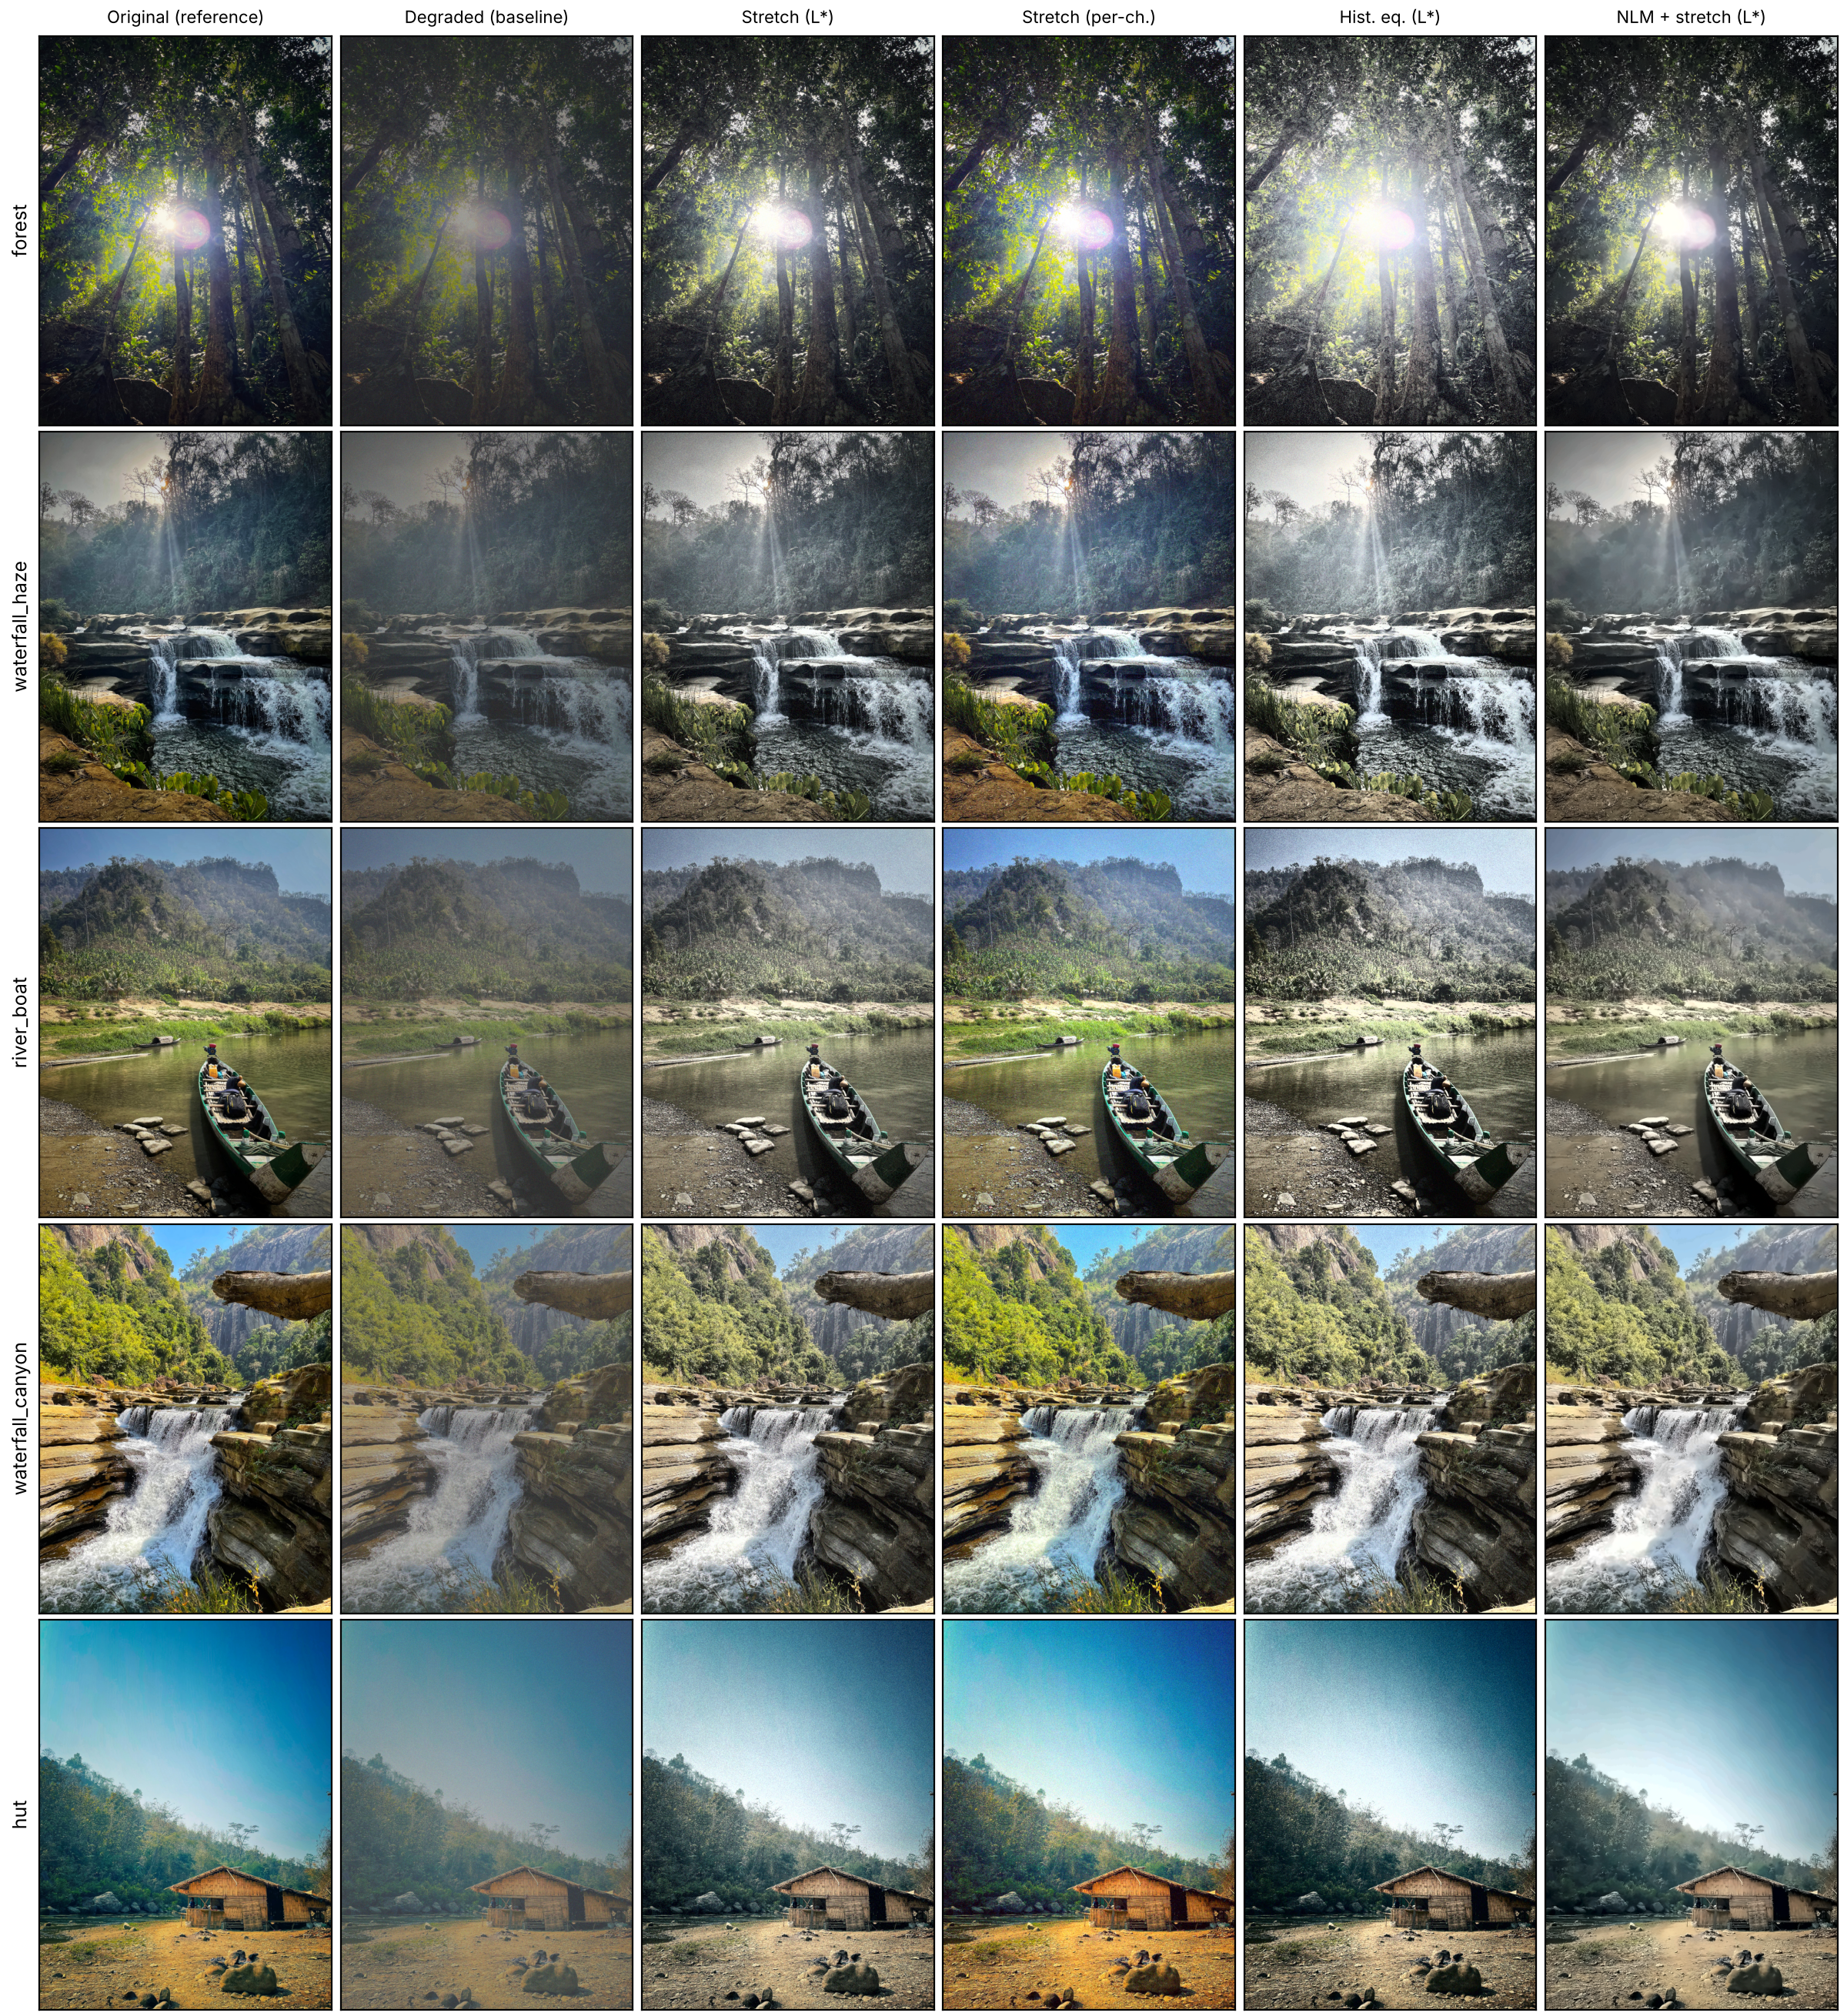
\includegraphics[width=0.93\linewidth]{comparison_grid.png}
\caption{Original (reference), degraded input (= baseline) and the four enhancement results for each image.}
\label{fig:grid}
\end{figure}

\begin{table}[!ht]
\centering\small
\caption{Metrics with respect to the original (higher PSNR/SSIM and lower MAE are better). Bold: best per image.}
\label{tab:m}
\begin{tabular}{@{}llccc@{}}
\toprule
Image & Method & PSNR [dB] $\uparrow$ & SSIM $\uparrow$ & MAE $\downarrow$\\\midrule
\multirow{5}{*}{\texttt{forest}} & Baseline (degraded) & 19.69 & 0.667 & 20.36 \\
 & Linear stretch, $L^*$ & 22.67 & 0.708 & 13.86 \\
 & Linear stretch, per channel & 22.25 & 0.622 & 15.97 \\
 & Hist.\ equalisation, $L^*$ & 11.29 & 0.412 & 61.21 \\
 & NLM + stretch, $L^*$ & \textbf{22.97} & \textbf{0.790} & \textbf{12.13} \\
\midrule
\multirow{5}{*}{\texttt{waterfall\_haze}} & Baseline (degraded) & 20.04 & 0.681 & 20.68 \\
 & Linear stretch, $L^*$ & 20.92 & 0.727 & 18.80 \\
 & Linear stretch, per channel & 19.66 & 0.635 & 22.40 \\
 & Hist.\ equalisation, $L^*$ & 13.92 & 0.598 & 42.90 \\
 & NLM + stretch, $L^*$ & \textbf{21.80} & \textbf{0.825} & \textbf{16.54} \\
\midrule
\multirow{5}{*}{\texttt{river\_boat}} & Baseline (degraded) & 20.36 & 0.693 & 19.58 \\
 & Linear stretch, $L^*$ & 19.79 & 0.721 & 21.64 \\
 & Linear stretch, per channel & 19.82 & 0.641 & 21.67 \\
 & Hist.\ equalisation, $L^*$ & 15.48 & 0.594 & 33.54 \\
 & NLM + stretch, $L^*$ & \textbf{20.44} & \textbf{0.823} & \textbf{19.43} \\
\midrule
\multirow{5}{*}{\texttt{waterfall\_canyon}} & Baseline (degraded) & 17.56 & 0.686 & 28.75 \\
 & Linear stretch, $L^*$ & 22.10 & \textbf{0.826} & 14.44 \\
 & Linear stretch, per channel & \textbf{25.04} & 0.791 & \textbf{11.40} \\
 & Hist.\ equalisation, $L^*$ & 19.68 & 0.806 & 19.83 \\
 & NLM + stretch, $L^*$ & 21.09 & 0.825 & 15.96 \\
\midrule
\multirow{5}{*}{\texttt{hut}} & Baseline (degraded) & 17.87 & 0.635 & 28.06 \\
 & Linear stretch, $L^*$ & 18.65 & 0.573 & 22.99 \\
 & Linear stretch, per channel & \textbf{21.36} & 0.514 & \textbf{17.92} \\
 & Hist.\ equalisation, $L^*$ & 17.62 & 0.524 & 27.62 \\
 & NLM + stretch, $L^*$ & 18.42 & \textbf{0.799} & 23.52 \\
\bottomrule
\end{tabular}
\end{table}

\begin{figure}[!ht]
\centering
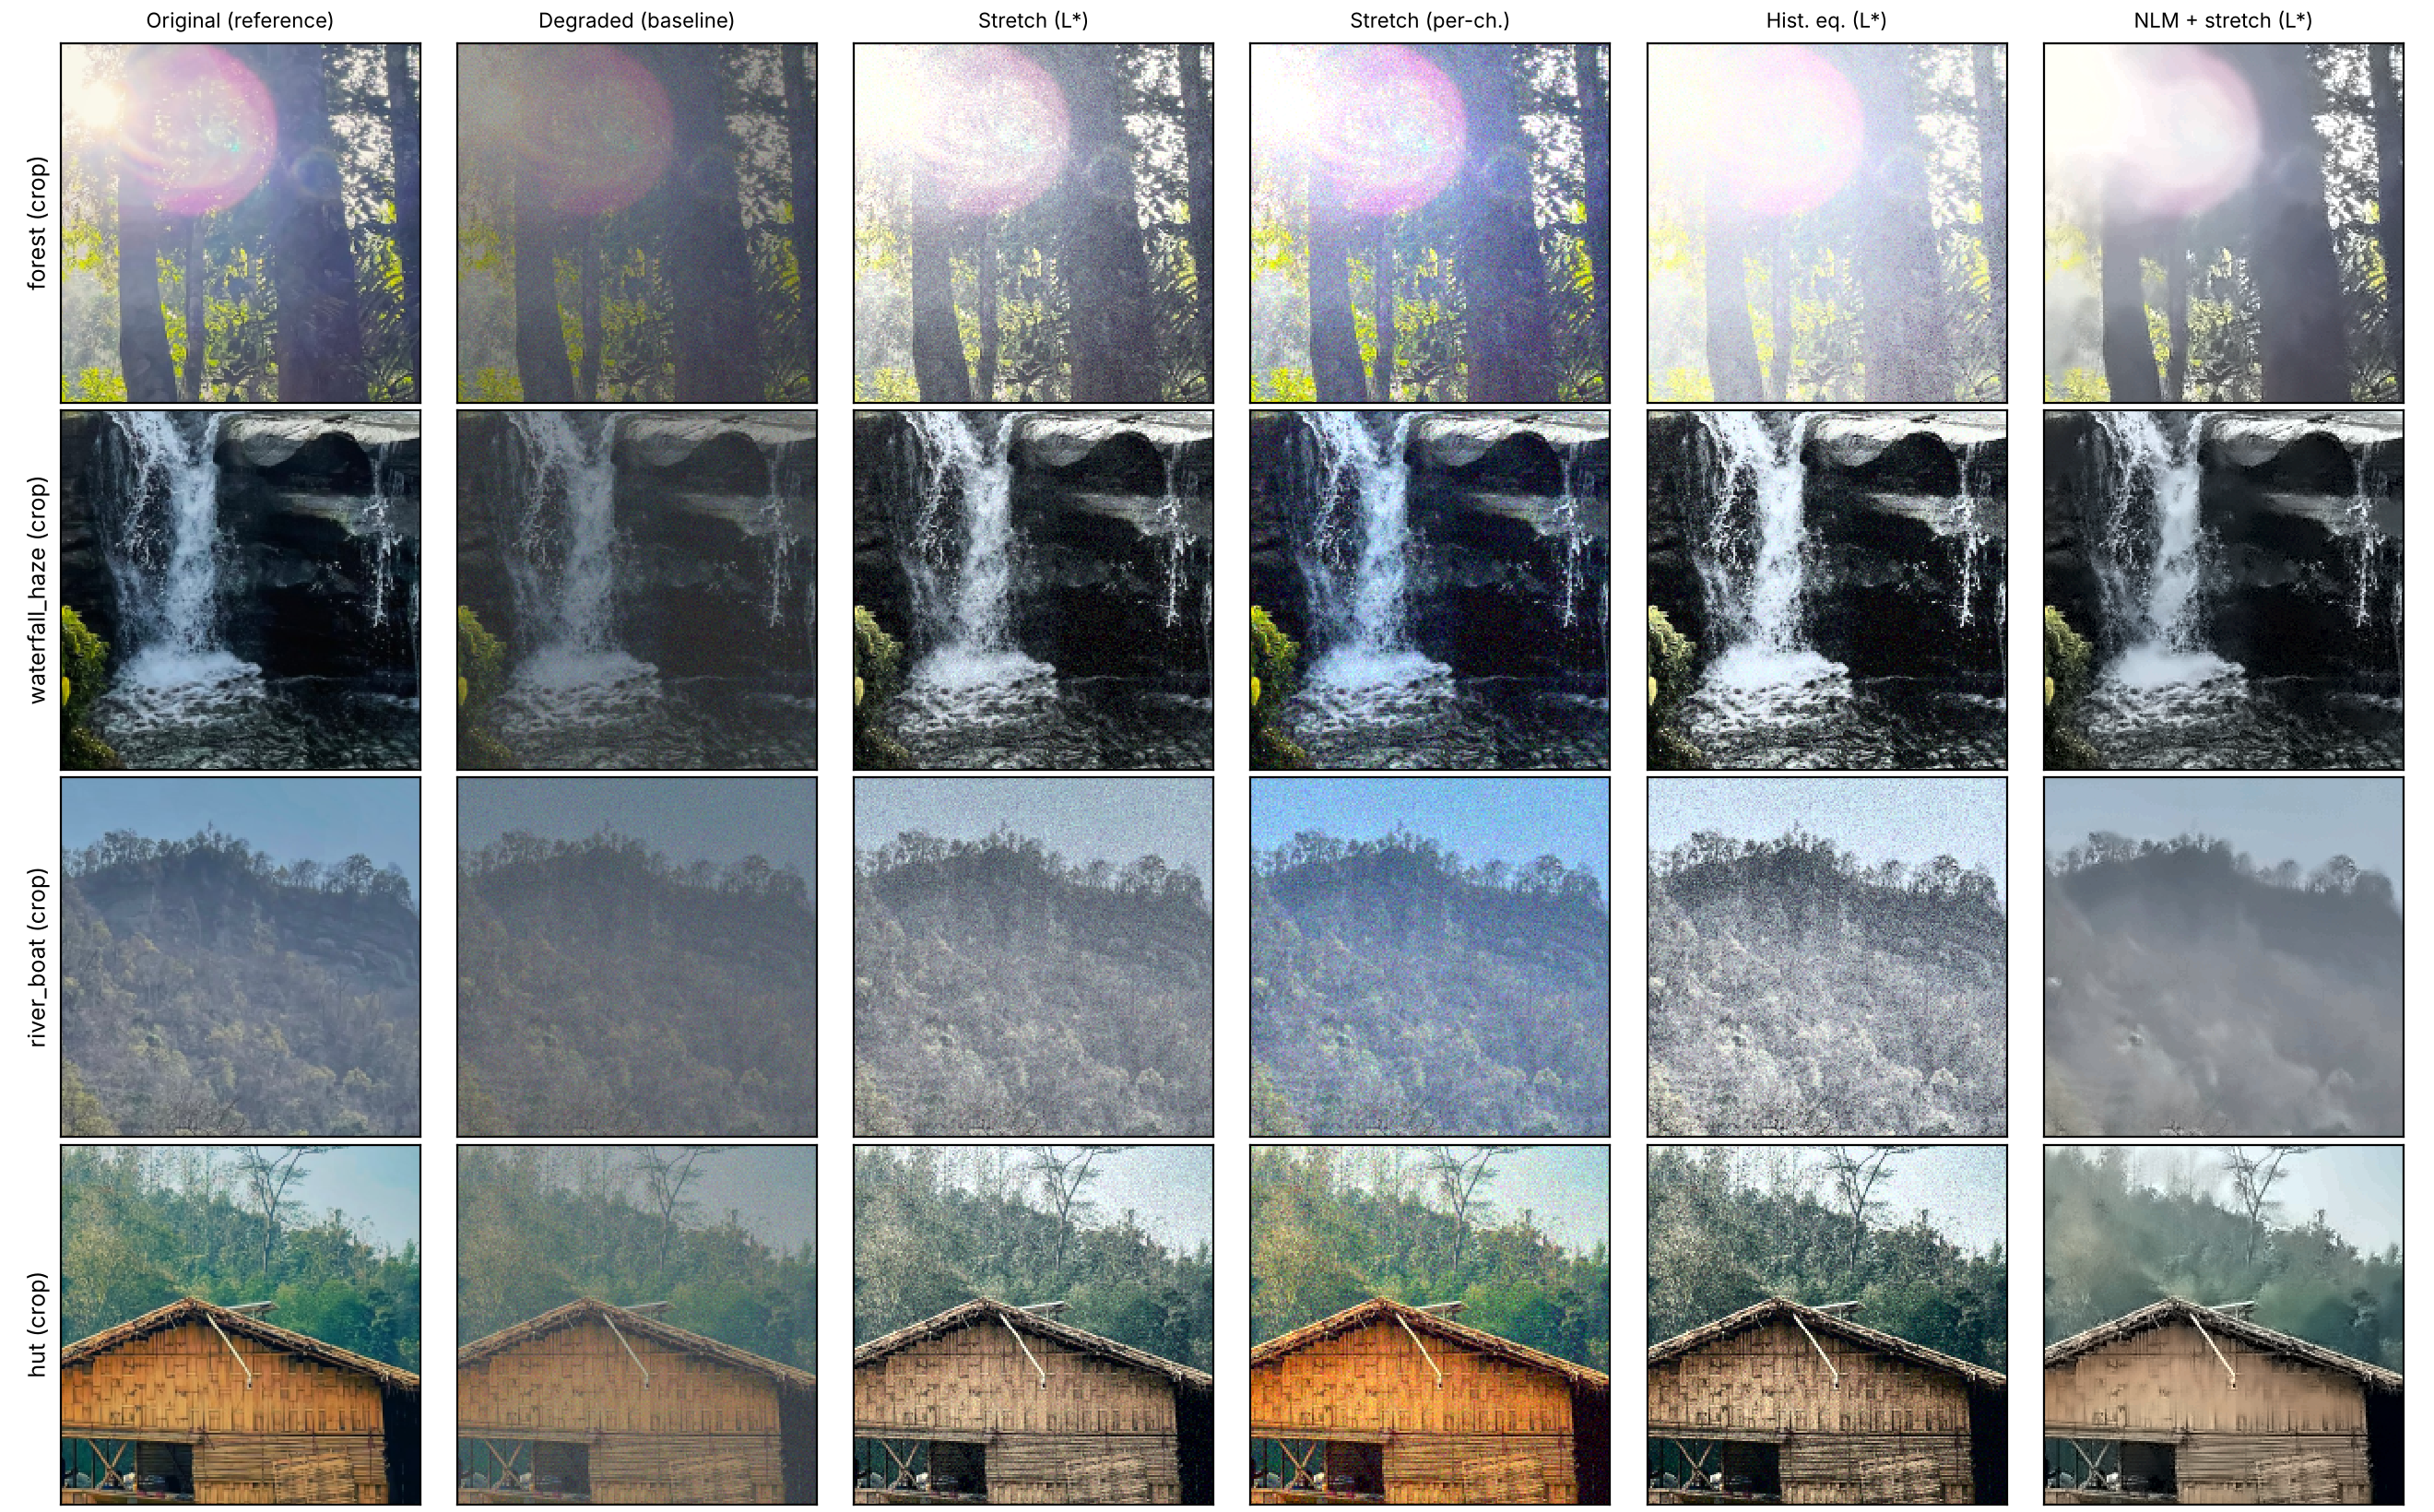
\includegraphics[width=\linewidth]{crops.png}
\caption{Zoomed crops (200$\times$200 px, nearest-neighbour): flare region of \texttt{forest}, falls of
\texttt{waterfall\_haze}, distant hillside of \texttt{river\_boat}, roof and hillside of \texttt{hut}.}
\label{fig:crops}
\end{figure}

\section{Discussion}
\textbf{General trends.} $L^*$ stretching improves PSNR over the baseline on four of the five images and
NLM+stretch on all five; histogram equalisation has the lowest PSNR on four of five. HE fails numerically because it forces a flat
$L^*$ histogram: the dark \texttt{forest} (mean $L^*$ 67/255) is lifted to mid-grey, and the large bright sun/flare
area grows into a big white blob (Fig.~\ref{fig:crops}, row 1). All stretching methods amplify the noise: in a flat
patch of the \texttt{hut} sky the high-frequency $L^*$ standard deviation goes from 4.7 (degraded) to 11.3 after
$L^*$ stretching and 16.1 after HE, but only 1.3 after NLM+stretch (original: 1.0). Consequently NLM+stretch has the
best SSIM on four of five images. Two systematic limits remain: (i) $L^*$-only methods cannot restore the
saturation removed by the degradation (mean chroma of \texttt{hut} stays at 14.8 vs.\ 25.0 originally), so the wooden
hut turns beige-grey instead of orange; (ii) all methods are global, so they do not remove haze locally or balance
the sunlit vs.\ shadowed parts of \texttt{waterfall\_canyon}; a local method (CLAHE, homomorphic filtering) would
be needed for that.

\textbf{Case 1 -- better numbers, worse-looking image (\texttt{hut}, per-channel stretch).} Per-channel stretching
gives the best PSNR (21.36\,dB) and MAE (17.92) on \texttt{hut} (and on \texttt{waterfall\_canyon}, 25.04\,dB),
because the independent channel gains also stretch the chroma and bring the orange wood and blue sky closer to the
reference. Yet it has the \emph{lowest SSIM of all methods} on \texttt{hut} (0.514), and the crop shows strong
\emph{coloured} grain on the roof and in the sky. PSNR/MAE are dominated by the large, low-frequency colour error,
whereas SSIM and the eye are sensitive to high-frequency noise. Per-channel gains also exaggerate colour:
on \texttt{forest} and \texttt{waterfall\_haze} the mean chroma becomes 17.4, against about 10 in the originals.

\textbf{Case 2 -- the ``best'' method erases detail (\texttt{river\_boat}, NLM+stretch).} NLM+stretch wins all three
metrics on \texttt{river\_boat} (PSNR 20.44, SSIM 0.823, MAE 19.43), but the crop of the distant hillside shows that
individual tree crowns have been smoothed into flat, painterly patches. The haze already makes this texture weak,
so after the contrast reduction its amplitude is comparable to the noise and NLM removes both. Plain $L^*$
stretching keeps the trees visible, at the price of grain, but has a \emph{lower PSNR than the unprocessed baseline}
(19.79 vs.\ 20.36\,dB): the 1--99\% stretch maps to the full $[0,255]$ range, while the original only spans
$[2,218]$ ($p_1$--$p_{99}$ of $L^*$), so the more contrasted result is counted as error. The reference-based
metrics measure \emph{restoration}, not \emph{enhancement}.

\textbf{Qualitative analysis.}
\emph{\texttt{forest}} -- preferred: \textbf{NLM+stretch} (also best on all metrics). Trunks, foliage and the
light rays come back, and the grain in the dark canopy is removed. Artifact: the flare area becomes slightly
blotchy with visible tone steps. HE reveals the most leaf detail in the shadows but floods the scene with a
yellow-white glow around the sun and lifts the shadows to an unnatural grey.
\emph{\texttt{waterfall\_haze}} -- preferred: \textbf{NLM+stretch} (best on all metrics). The water texture and rock
edges stay sharp because they are high-contrast structures that NLM preserves; the haze and sun rays remain
natural. HE makes the haze milky-white and noticeably noisier.
\emph{\texttt{hut}} -- no method is fully satisfying: $L^*$ stretching restores the contrast of the hillside but
desaturates the wood; per-channel stretching restores the colour but adds colour noise; NLM+stretch gives a clean
sky but smears the foliage on the hillside into a watercolour look (Fig.~\ref{fig:crops}, last row). Here we
prefer $L^*$ stretching for its natural appearance and visible detail.

\textbf{Real images, no reference.} Applying the methods directly to the original photographs
(Fig.~\ref{fig:real}; files \texttt{*\_REAL\_*} in \texttt{results/images/}) is the realistic case. $L^*$ stretching changes them only
mildly, since they already span most of the range. HE gives the strongest effect: it brings out texture in the hazy
forest of \texttt{waterfall\_haze} and on the \texttt{river\_boat} hillside, but over-brightens \texttt{forest},
spreading the sun glare over the canopy, and darkens the hillside of \texttt{hut}.

\begin{figure}[!ht]
\centering
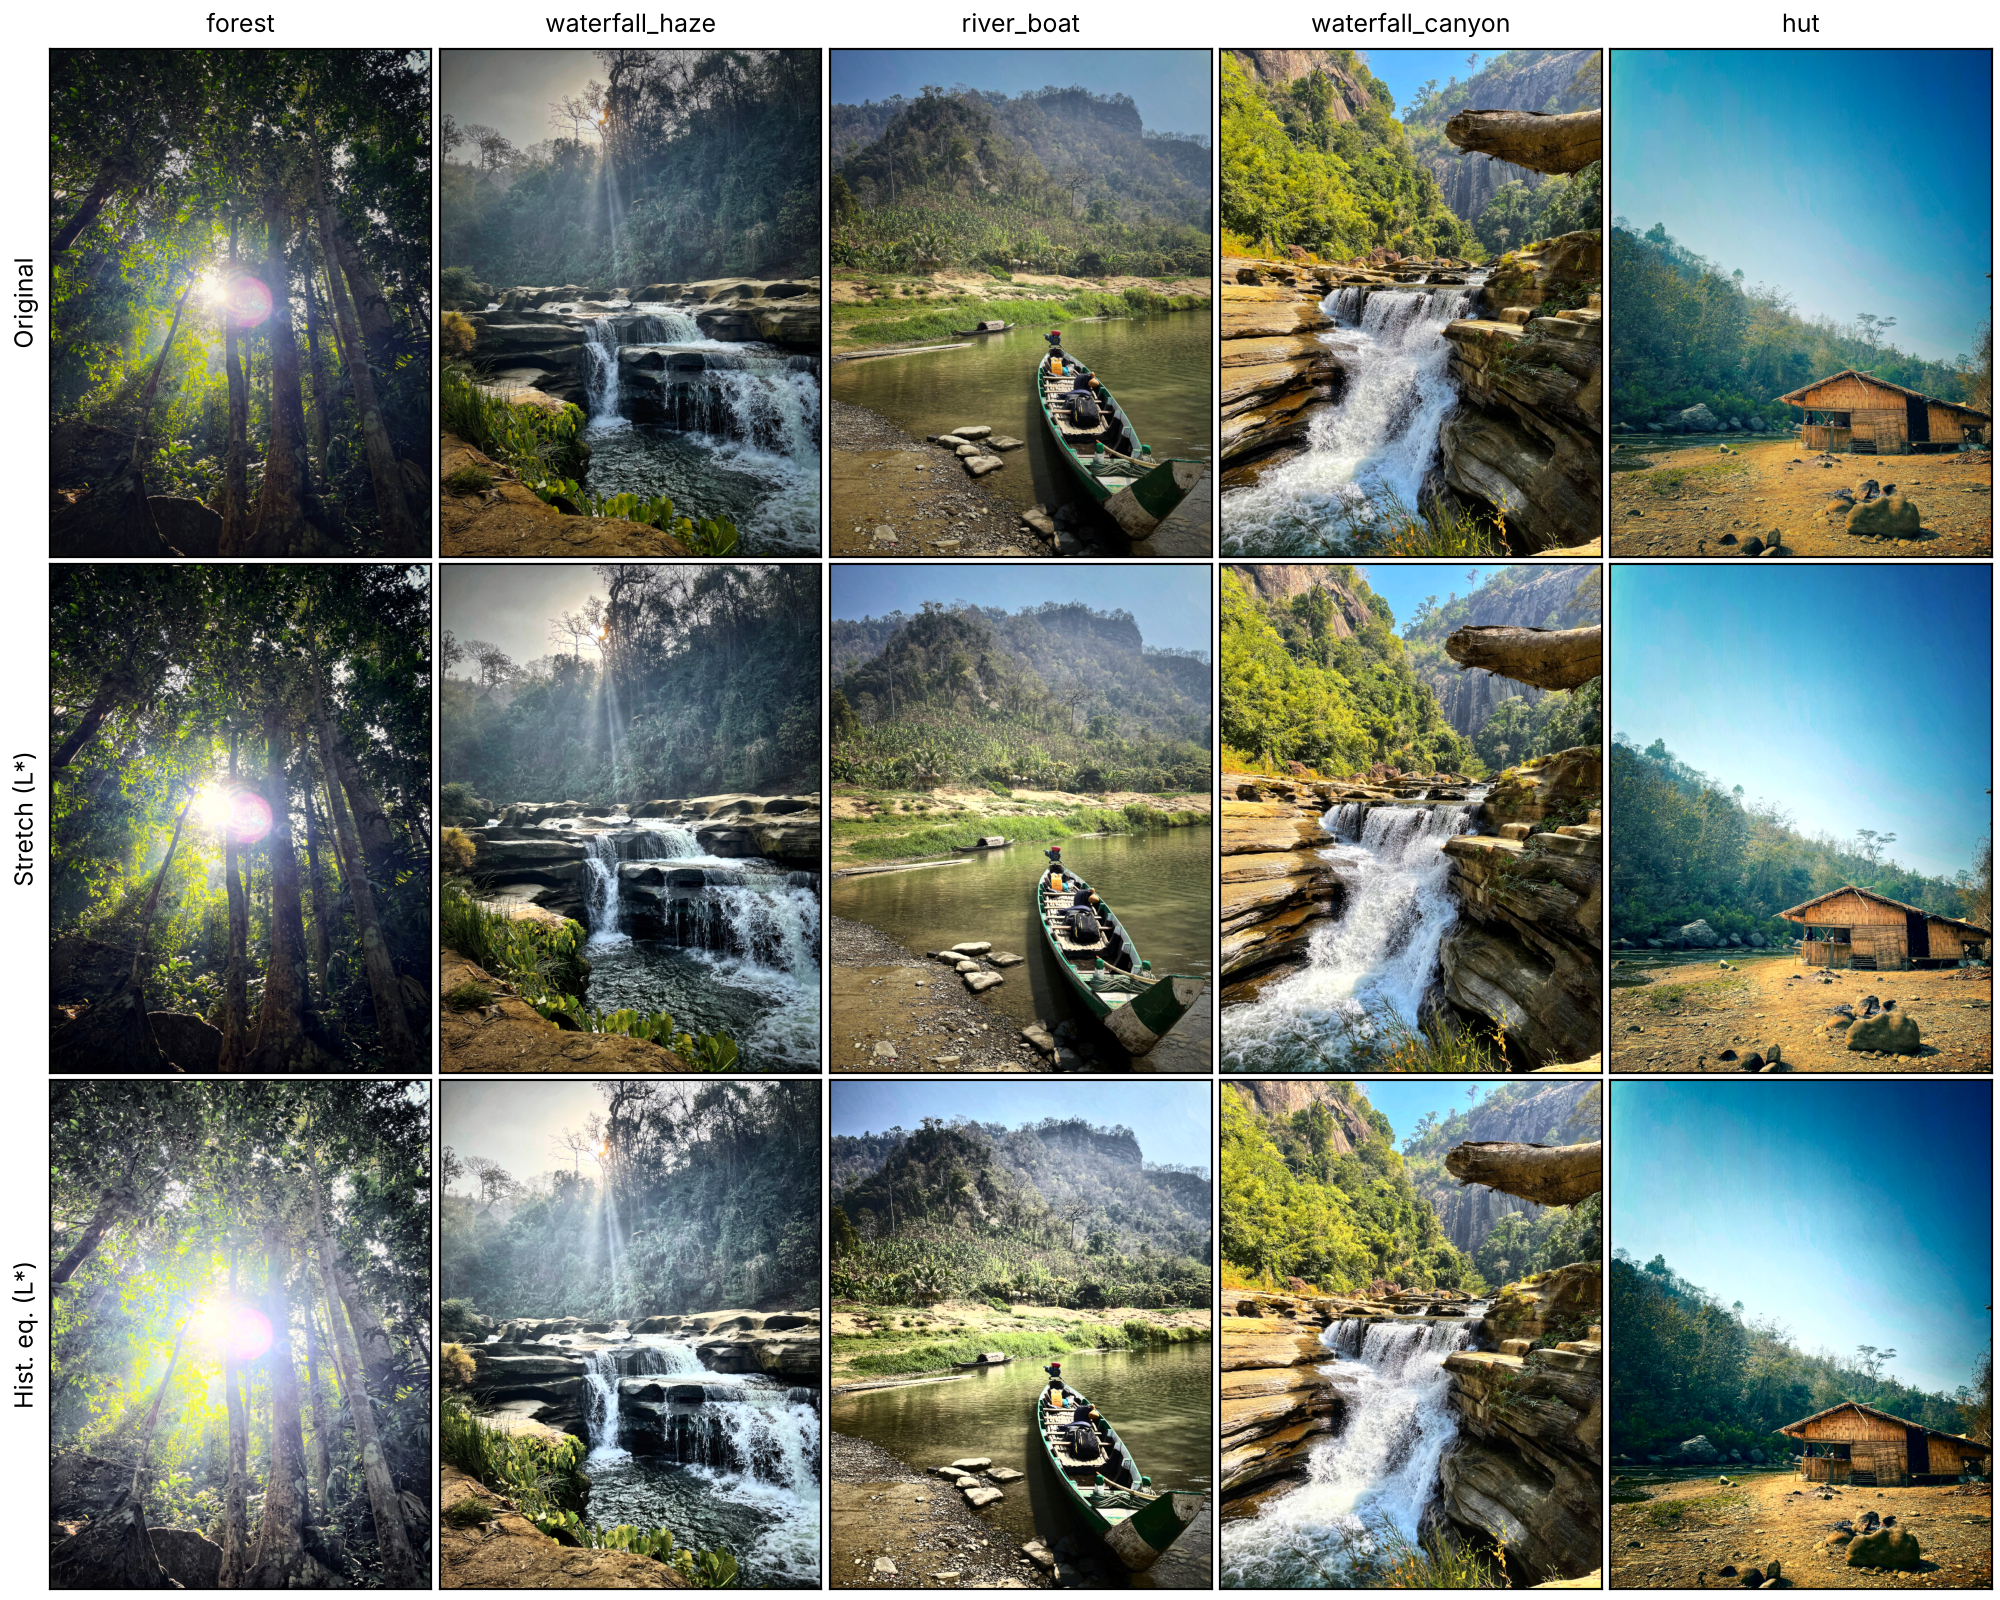
\includegraphics[width=0.62\linewidth]{real_no_reference.png}
\caption{Methods applied to the original photographs (no reference available).}
\label{fig:real}
\end{figure}

\textbf{Limitations.} The degradation is global with simple Gaussian noise (real low-light noise is
signal-dependent); one parameter setting per method is reported; the photographs were downsampled; and all metrics
are full-reference fidelity measures that do not capture visual pleasantness. We therefore do not pick a method
on a single metric: our default is \emph{NLM + luminance stretch} for noisy inputs, and plain luminance stretching
when fine, low-contrast texture (distant foliage) matters more than grain.

\begin{thebibliography}{9}\small
\bibitem{buades2005} A.~Buades, B.~Coll, J.-M.~Morel. A non-local algorithm for image denoising. \emph{CVPR}, 2005.
\bibitem{wang2004} Z.~Wang, A.~C.~Bovik, H.~R.~Sheikh, E.~P.~Simoncelli. Image quality assessment: from error
visibility to structural similarity. \emph{IEEE Trans.\ Image Processing}, 13(4), 2004.
\bibitem{skimage} S.~van der Walt et al. scikit-image: image processing in Python. \emph{PeerJ} 2:e453, 2014.
\bibitem{opencv} G.~Bradski. The OpenCV Library. \emph{Dr.\ Dobb's Journal of Software Tools}, 2000.
\bibitem{gw} R.~C.~Gonzalez, R.~E.~Woods. \emph{Digital Image Processing}, 4th ed. Pearson, 2018.
\end{thebibliography}
\end{document}
